% -*- root: ../../main.tex -*
%!TEX root = ../../main.tex
% vim:textwidth=80 fo=cqt conceallevel=0


At the outset, it is worth mentioning that the focus of this chapter
is on the layer optimisation \emph{methodology} itself. The results as
such do not stand alone outside of the modelling universe with all the
inherent assumptions discussed thus far. Presently, the value added by
this work is its ready adaptability to industry through its modular
design. A numerical implementation in the form of a toolbox\footnote{The
\gls{bold} Toolbox is made available for download from GitHub. \\
\mbox{\href{https://github.com/ImperialCollegeESE/BOLD_Toolbox}{
\includegraphics
[width=0.025\textwidth]{github.pdf}}} \url{
https://github.com/ImperialCollegeESE/BOLD_Toolbox}} is also provided which
is immediately available for download and use by industry. This author
recommends that until the tool matures, cell manufacturers substitute their own
parameters and adjust other numerical coefficients suitably so that the toolbox
supplements, rather than supplants their empirical layer designs. Hence, the
results presented in this section must be interpreted in the backdrop of the
context within which the methodology was developed implying that the reader
must consciously strive to interpret all numerical values in relative terms of
magnitude. To aid this thought process, this author chooses to deliberately
limit the discussion on the absolute magnitude of numbers presented here.

%\subsection{Modelling Platform and Preconditioning}

%Couple of statements  about why LIONSIMBA was chosen as  the modelling platform
%for implementing the p2d dynamics. The  cell parameters used are shown in table
%xx. This cell is henceforth known as the LIONSIMBA cell or Northrop cell.

%Discuss the  missing elements  in LIONSIMBA  only with  respect to  the present
%problem at hand, \viz{the stoichiometries}.

%%\subsubsection*{Stoichiometry Augmentation}

%%Discuss the problem first. How LIONSIMBA started always at 85.51 percentage and
%%needed to  do a  discharge down to  zero percent before  having the  ability to
%%charge. For this project, stoichiometries  are vital for capacity determination
%%and  the 1C  current density.  Explain how  stoichiometries were  refined until
%%cut-off for  infinitesimal bleeding discharge current  achieved. Noted relevant
%%values. Explain refinement  of how approximate capacities  reported by Northrop
%%and Subramanian were  refined precisely. Explanation of  remnant capacities and
%%stoichiometries computation. Explanation of  1C current density.parameters init
%%capacity computation code.

%%% -*- root: ../../main.tex -*-
%!TEX root = ../../main.tex
% vim:nospell

\begin{table}[!htbp]
    \small
    \caption[%
    System-level simulation conditions \& thermal parameters of  an \glsfmtshort{lco} cell
    ]%
    {%
        Cell   parameters   and   system   conditions  for   a   simulating   an
        \glsfmtshort{lco} cell  with the  \gls{dfn} electrochemical model  and a
        lumped thermal model. The parameters  presented here when augmented with
        the  values  of  the  kinetic, geometric  and  transport  properties  of
        the  cell (from  \cref{tbl:lcoSimParamsSPMp2d}  represents the  complete
        information  required for  all  simulations in  this layer  optimisation
        framework.
    }%
    \label{tbl:lcoSimParamslayeropt}
    \vspace{-2.6229525pt}
    \begin{threeparttable}
        \centering
        \textbf{System Conditions} \\ \smallskip
        \begin{varwidth}[t]{0.48\linewidth}
            \begin{tabular*}{\textwidth}{@{} l @{\extracolsep{\fill}} S[table-format=1.2,table-space-text-pre=\Tnote{a} ,table-align-text-pre=false] @{}}
                \toprule
                \multicolumn{1}{@{}l}{Parameter} \\
                \midrule

                Lower cutoff cell voltage, $V_\text{min}$ (\si{\volt}) & \Tnote{a} 3.50   \\
                Upper cutoff cell voltage, $V_\text{max}$ (\si{\volt}) & \Tnote{b} 4.22   \\

                \bottomrule
            \end{tabular*}
        \end{varwidth}
        \hfill
        \begin{varwidth}[t]{0.48\linewidth}
            \begin{tabular*}{\textwidth}{@{} l @{\extracolsep{\fill}} S[table-format=2.2,table-space-text-pre=\Tnote{a} ,table-align-text-pre=false] @{}}
                \toprule
                \multicolumn{1}{@{}l}{Parameter} \\
                \midrule

                Target cell SOC for fast charge, $z^\ast$ \si{(\%)}                & \Tnote{c} 80.00 \\
                Cell upper temperature limit, $T_\text{max}$ \si{(\degreeCelsius)} & \Tnote{d} 55.00 \\

                \bottomrule
            \end{tabular*}
        \end{varwidth}

        \medskip
        \begin{tabular*}{\textwidth}{@{} l @{\extracolsep{\fill}} r @{}}
            \multicolumn{2}{c}{\textbf{Geometric Parameters}} \\
            \toprule
            \multicolumn{1}{@{}l}{Parameter} \\
            \midrule
            Surface area of pos.\ \& neg.\ electrode overlap within a layer, {$A_\text{elec}$} \si{(m^2)} & \textsuperscript{b}\num{4.19e-2}   \\
            Exterior pouch length, $L_\text{pouch}$ \si{(m)}                                              & \textsuperscript{e}\num{332.74e-3} \\
            Exterior pouch width, $W_\text{pouch}$ \si{(m)}                                               & \textsuperscript{e}\num{99.06e-3}  \\
            Exterior pouch height, $H_\text{pouch}$ \si{(m)}                                              & \textsuperscript{f}\num{10.00e-3}  \\
            Pouch material thickness, $T_\text{pouch}$ \si{(m)}                                           & \textsuperscript{g}\num{160.00e-6} \\
            \bottomrule
        \end{tabular*}
        \medskip
        \centering \textbf{Thermal Parameters} \\ \smallskip
        \resizebox{\textwidth}{!}{%
            \begin{tabular}{@{} l S[table-format=4.0,table-space-text-pre=\Tnote{m} ,table-align-text-pre=false] S[table-format=4.1,table-space-text-pre=\Tnote{m} ,table-align-text-pre=false] S[table-format=4.1,table-space-text-pre=\Tnote{m} ,table-align-text-pre=false] S[table-format=4.2,table-space-text-pre=\Tnote{m} ,table-align-text-pre=false] S[table-format=4.0,table-space-text-pre=\Tnote{m} ,table-align-text-pre=false] S[table-format=4.1,table-space-text-pre=\Tnote{m} ,table-align-text-pre=false] S[table-format=4.1,table-space-text-pre=\Tnote{m} ,table-align-text-pre=false] @{}}
                \toprule
                \multicolumn{1}{@{}l}{Parameter} & \multicolumn{1}{c}{Al.\ CC} & \multicolumn{1}{c}{Pos} & \multicolumn{1}{c}{Sep} & \multicolumn{1}{c}{Neg} & \multicolumn{1}{c}{Cu.\ CC} & \multicolumn{1}{c}{\ch{LiPF_6}} & \multicolumn{1}{r@{}}{Pouch}\\
                \midrule

                Sp.\ heat capacity, $c_j$ (\si{\joule\per\kilogram\per\kelvin})   & \Tnote{h} 903  & \Tnote{h} 1269.2 & \Tnote{h} 1978.2 & \Tnote{h} 1437.4 & \Tnote{h} 385  & \Tnote{h} 2055.1 & \Tnote{i} 1464.8 \\
                Density, $\rho_j$ (\si{\kilogram\per\meter\cubed})                & \Tnote{j} 2700 & \Tnote{k} 2291.6 & \Tnote{b} 1100.0 & \Tnote{j} 2660.0 & \Tnote{l} 8960 & \Tnote{j} 1290.0 & \Tnote{m} 1150.0 \\
                Activ.\ energy, diff. ${E_\text{act,s}}_j$ (\si{\joule\per\mole}) & {---}                   & \Tnote{p} 5000   & {---}                     & \Tnote{p} 5000   & {---}                   & {---}                     & \multicolumn{1}{c}{---}   \\
                Activ.\ energy, rxn. ${E_\text{act,k}}_j$ (\si{\joule\per\mole})  & {---}                   & \Tnote{p} 5000   & {---}                     & \Tnote{p} 5000   & {---}                   & {---}                     & \multicolumn{1}{c}{---}   \\

                \bottomrule
            \end{tabular}
        }
        \medskip
        \begin{tabular*}{\textwidth}{@{} l @{\extracolsep{\fill}} r @{}}
            \multicolumn{2}{c}{\textbf{Other Geometric/Cell-Level Parameters}} \\
            \toprule
            \multicolumn{1}{@{}l}{Parameter} \\
            \midrule

            Thickness of pos.\ current collector, $l_\text{Al}$ \si{(m)}                    & \textsuperscript{f}\num{15e-6}   \\
            Thickness of neg.\ current collector, $l_\text{Cu}$ \si{(m)}                    & \textsuperscript{p}\num{10e-6}   \\
            Total tab area, $A_\text{tabs}$ \si{(m^2)}                                      & \textsuperscript{b}\num{5.94e-3} \\
            Lumped heat transfer coefficient, $h$ (\si{\watt\per\meter\squared\per\kelvin}) & \textsuperscript{b}150           \\
            Initial electrolyte concentration, $c_\text{e,0}$ (\si{\mole\per\meter\cubed})  & \textsuperscript{q}1000          \\

            \bottomrule
        \end{tabular*}

        \medskip
        \begin{tabular*}{\textwidth}{@{} =P{7.5cm}  +l@{\extracolsep{\fill}}+c +r @{}}
            \multicolumn{4}{c}{\textbf{Spatial Discretisation}} \\
            \toprule
            \multicolumn{1}{@{}l}{Parameter} & \multicolumn{1}{l}{Pos} & \multicolumn{1}{c}{Sep} & \multicolumn{1}{r@{}}{Neg}\\
            \midrule

            Nodes, through-thickness (axial), $N_{\text{a}_j}$          & \num{40} & \num{40} & \num{40} \\
            Nodes, within spherical particle (radial), $N_{\text{r}_j}$ & \num{15} & ---      & \num{15} \\

            \bottomrule
        \end{tabular*}

        \medskip
        \vspace{-2.6229525pt}
        \begin{tablenotes}[para,flushleft]
            \begin{footnotesize}
            \item[a] Calculated as described in \cref{sec:cutoff}
            \item[b] Assumed
            \item[c] Ref.~\cite{Sae2010}
            \item[d] Ref.~\cite{Kizilel2009} \\
            \item[e] Converted from imperial units reported in~Ref.~\cite{GMBoltBatteryDims}
		    \item[f] Table~\romanletter{4} of~Ref.~\cite{Groger2015} \\
            \item[g] Sum of values in table~1 of~Ref.~\cite{Svens2013}
            \item[h] Ref.~\cite{Chen2005}
            \item[i] Computed from values of constituents (see~\cite{Svens2013}) using Ref.~\cite{martienssen2006springer} \\
            \item[j] Ref.~\cite{Guo2010}
            \item[k] Ref.~\cite{Jeon2011}
            \item[l] Ref.~\cite{Worwood2017,Song2000}
            \item[m] Ref.~\cite{Kim2009}
            \item[p] Ref.~\cite{Northrop2011}
            \item[q] Ref.~\cite{Subramanian2009}
            \end{footnotesize}
        \end{tablenotes}
    \end{threeparttable}
\end{table}


%%%% -*- root: ../../main.tex -*-
%!TEX root = ../../main.tex
% vim:nospell


\begin{table}[!htbp]
	\renewcommand{\thetable}{\arabic{table}a}
	\centering
	\caption{Acceleration test parameters (common across xEV platforms)}
	\label{tbl:CommonVehicleParams}
	\sisetup{table-format=3.2, table-number-alignment=center, table-space-text-pre=\textsuperscript{a}, table-space-text-post=\textsuperscript{a}, table-align-text-post=false}
	\begin{threeparttable}[t]
		\centering
		\begin{tabular}{@{} l  S @{}}
			\toprule
			Parameter \\
			\midrule

			% Coefficient of drag for xEV body, $C_\mathrm{d}$                           & {\makebox*{00}[r]{\tnote{a}}} 0.31                \\
			% Frontal area of xEV, $A_\mathrm{v}$ \si{(m^2)}                             & {\makebox*{00}[r]{\tnote{b}}} 2.40                \\
			% Acc.\ time specified by manufacturer, $t_\mathrm{f,man}$ \si{(s)}          & {\makebox*{00}[r]{\tnote{d}}} 6.50                \\
			% Acc.\ time dictated by standards, $t_\mathrm{f,std}$ \si{(s)}              & {\makebox*{00}[r]{\tnote{c}}} 6.00                \\
			% Speed, end of acc. (standards), $v_\mathrm{f,std}$ \si{(m.s^{-1})}         & {\makebox*{00}[r]{\tnote{e}}} 8.94                \\
			% Speed, end of acc. (manufacturer), $v_\mathrm{f,man}$ \si{(m.s^{-1})}      & {\makebox*{0}[r]{\tnote{f}}} 26.82                \\
			% Base speed of  xEV, $v_\mathrm{b}$ \si{(m.s^{-1})}                         & {\makebox*{\hspace*{0.5mm}0}[r]{\tnote{e}}} 13.41 \\
			% Air density at acc.\ test conditions, $\rho_\mathrm{air}$ \si{(kg.m^{-3})} & {\makebox*{\hspace*{0.5mm}00}[r]{\tnote{f}}} 1.20 \\
			% Drivetrain efficiency, $\eta_\mathrm{dt}$                                  & {\makebox*{00}[r]{\tnote{g}}} 0.75                \\
			% Payload, $M_\mathrm{p}$ \si{(kg)}                                          & {\hspace*{0.00005mm}{\tnote{c}}} 150.60 \\
			% Rolling resistance coefficient of road surface, $C_\mathrm{r}$             & {\makebox*{00}[r]{\tnote{f}}} 0.01                \\
			% Road gradient, $Z$                                                         & {\makebox*{00}[r]{\tnote{g}}} 0.00                \\

			Coefficient of drag for xEV body, $C_\mathrm{d}$                           & 0.31   {\tnote{a}} \\
			Frontal area of xEV, $A_\mathrm{v}$ \si{(m^2)}                             & 2.40   {\tnote{b}} \\
			Acc.\ time specified by manufacturer, $t_\mathrm{f,man}$ \si{(s)}          & 6.50   {\tnote{d}} \\
			Acc.\ time dictated by standards, $t_\mathrm{f,std}$ \si{(s)}              & 6.00   {\tnote{c}} \\
			Speed, end of acc. (standards), $v_\mathrm{f,std}$ \si{(m.s^{-1})}         & 8.94   {\tnote{e}} \\
			Speed, end of acc. (manufacturer), $v_\mathrm{f,man}$ \si{(m.s^{-1})}      & 26.82  {\tnote{f}} \\
			Base speed of  xEV, $v_\mathrm{b}$ \si{(m.s^{-1})}                         & 13.41  {\tnote{e}} \\
			Air density at acc.\ test conditions, $\rho_\mathrm{air}$ \si{(kg.m^{-3})} & 1.20   {\tnote{f}} \\
			Drivetrain efficiency, $\eta_\mathrm{dt}$                                  & 0.75   {\tnote{g}} \\
			Payload, $M_\mathrm{p}$ \si{(kg)}                                          & 150.60 {\tnote{c}} \\
			Rolling resistance coefficient of road surface, $C_\mathrm{r}$             & 0.01   {\tnote{f}} \\
			Road gradient, $Z$                                                         & 0.00   {\tnote{g}} \\

			\bottomrule
		\end{tabular}
        \begin{tablenotes}[para,flushleft]
        \item[a]Ref.~\cite{HybridCars2017Drag}
        \item[b]Calculated from typical \gls{bev} dimensions in~\cite{BoltDimensions}
        \item[c]Ref.~\cite{ETANTP002-2004}
        \item[d]Ref.~\cite{BoltOverview}
        \item[e]Ref.~\cite{Liu2016a}
        \item[f]Ref.~\cite{EmadiElectric}
        \item[g]Assumed
        \end{tablenotes}
	\end{threeparttable}
\end{table}

%%%% -*- root: ../../main.tex -*-
%!TEX root = ../../main.tex
% vim:nospell


\begin{table}[!htbp] % Parameters unique to each of the BEV & PHEV
	% \addtocounter{table}{-1}
	% \renewcommand{\thetable}{\arabic{table}b}
	\caption{Acceleration test parameters (specific to each \glsfmtshort{xeV})}
	\label{tbl:UniqueVehicleParams}
	\centering
    \sisetup{table-format=4.1, table-number-alignment=center, table-space-text-pre=\textsuperscript{a}, table-align-text-pre=false}
	\begin{threeparttable}[t]
		\begin{tabular*}{0.72\textwidth}{@{} l @{\extracolsep{\fill}}  S S @{}}	% Works with Tnote
			\toprule
			\multicolumn{1}{@{} l}{Parameter} & \multicolumn{1}{c}{BEV} & \multicolumn{1}{c@{}}{PHEV} \\
			\midrule

			Mass of xEV chassis, $M_\mathrm{c}$ \si{(kg)}               & \Tnote{a} 1340.0 & \Tnote{b} 1438.0 \\
			Mass of pack overhead (w/o cells), $M_\mathrm{o}$ \si{(kg)} & \Tnote{a} 196.4  & \Tnote{c} 65.5   \\
			Upper cutoff SOC of cell, $z_\mathrm{max}$ \si{(\%)}        & \Tnote{d} 95.0   & \Tnote{d} 90.0   \\
			Lower cutoff SOC of cell, $z_\mathrm{min}$ \si{(\%)}        & \Tnote{d} 5.0    & \Tnote{e} 30.0   \\

			\bottomrule
		\end{tabular*}
		\begin{tablenotes}[para,flushleft]
		\item[a]Calculated based on~\cite{ChevyBoltSpecs}
		\item[b]Calculated based on~\cite{motortrendEcotec,ChevyBoltSpecs}
		\item[c]Calculated (see sections~\ref{sec:layerdependentvehiclemass} \& \ref{sec:massofonecell})
		\item[d]Assumed
		\item[e]Ref.~\cite{EmadiElectric}
		\end{tablenotes}

	\end{threeparttable}
\end{table}

%%%% -*- root: ../../main.tex -*-
%!TEX root = ../../main.tex
% vim:nospell

\begin{table}[htb!]
    \caption{\glsfmtshort{xeV} acceleration test results}
    \label{tbl:accResults}
    \centering
	\begin{tabular}{c c c}
        \toprule
        \multicolumn{1}{@{} l}{\makecell{($T_\text{init},T_\text{sink}$) \\ \footnotesize (degC)}} & \makecell{$n^\text{acc}_\text{opt}$ \\ \footnotesize \glsfmtshort{bev}}&  \multicolumn{1}{c @{}}{\makecell{$n^\text{acc}_\text{opt}$ \\ \footnotesize \gls{phev}}}  \\
        \midrule

        (38,5)  & \num{21} & \num{55} \\
        (38,49) & \num{21} & \num{57} \\
        (25,25) & \num{23} & \num{63} \\
        (15,5)  & \num{27} & \num{69} \\

        \bottomrule
    \end{tabular}
\end{table}


%%\begin{figure}[!bp]
%%    \begin{minipage}[t]{\textwidth}
%%        \centering
%%        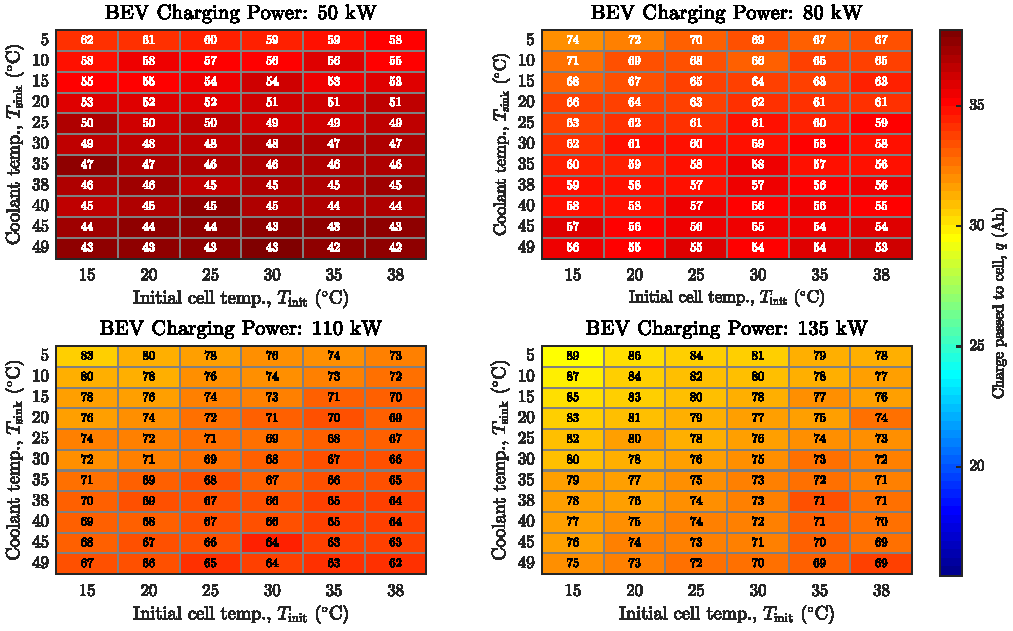
\includegraphics[width=\textwidth]{fig_generate_heatmap_BEV}
%%        \captionsetup{labelsep=note}
%%        \caption[Optimal cell layer configurations for the \gls{bev}, presented for a range of fast charging powers and thermal conditions]{Optimal cell layer configurations for the \gls{bev}, presented for a range of fast charging powers and thermal conditions.}
%%        \label{fig:fig_generate_heatmap_BEV}
%%        \mpfootnotes[1]
%%        \footnote{This figure was created by \mbox{Ian Campbell} who asserts copyright,
%%            with intellectual contributions from and the right to use asserted by
%%        \mbox{Krishnakumar Gopalakrishnan}.}
%%    \end{minipage}
%%\end{figure}

%%\begin{figure*}[!bp]
%%    \begin{minipage}[t]{\textwidth}
%%        \centering 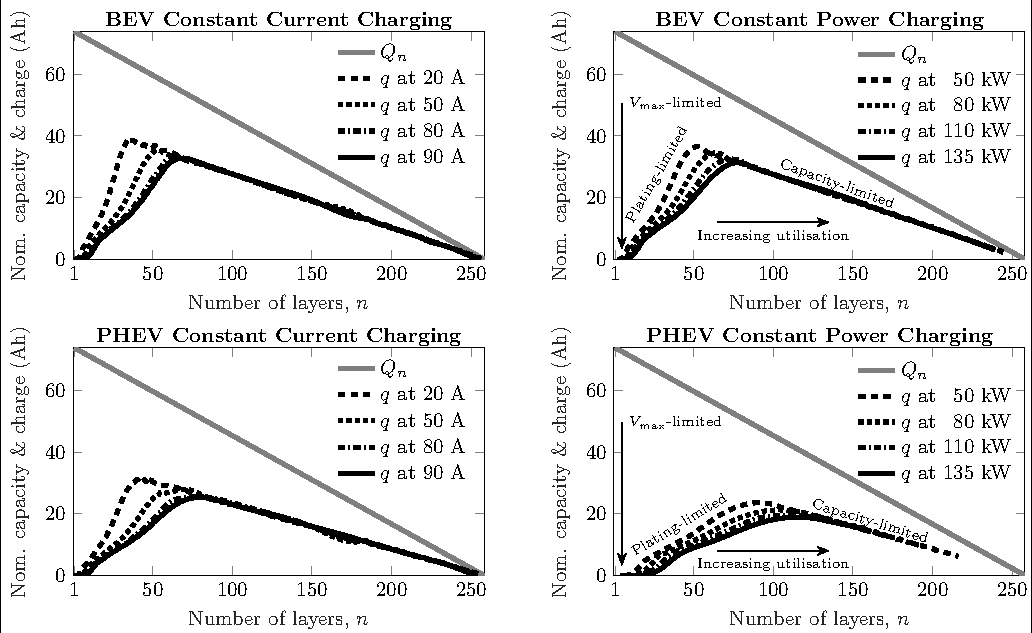
\includegraphics[width=\textwidth,trim=4 2 3 4,clip]{fig_capacity_quadrants.pdf}
%%        \captionsetup{labelsep=note}
%%        \caption[The plots in the right column show the nominal cell capacity and charge passed
%%        during \gls{xeV} \gls{cp} charging. Increased rate capability and cell utilisation are positively
%%        correlated with $n$, while the maximum-$q$ layer configuration clearly shifts to higher
%%        values of $n$ with increasing charging powers. The plots in the left column depict
%%        galvanostatic charging scenarios at various currents to highlight the similarity with the
%%        \gls{cp} process. All data obtained at $T_\text{init} =$ \SI{25}{\degreeCelsius},
%%        $T_\text{sink} =$ \SI{25}{\degreeCelsius}.]{The plots in the right column show the nominal cell capacity and charge passed
%%            during \gls{xeV} \gls{cp} charging. Increased rate capability and cell utilisation are positively
%%            correlated with $n$, while the maximum-$q$ layer configuration clearly shifts to higher
%%            values of $n$ with increasing charging powers. The plots in the left column depict
%%            galvanostatic charging scenarios at various currents to highlight the similarity with the
%%            \gls{cp} process. All data obtained at $T_\text{init} =$ \SI{25}{\degreeCelsius},
%%        $T_\text{sink} =$ \SI{25}{\degreeCelsius}.}
%%        \label{fig:fig_CapacityQuadrants}
%%        \mpfootnotes[1]
%%        \footnote{This figure was created by \mbox{Ian Campbell} who asserts copyright,
%%            with intellectual contributions from and the right to use asserted by
%%        \mbox{Krishnakumar Gopalakrishnan}.}
%%    \end{minipage}
%%\end{figure*}


%%\begin{figure}[!bp]
%%    \begin{minipage}[t]{\textwidth}
%%        \centering
%%        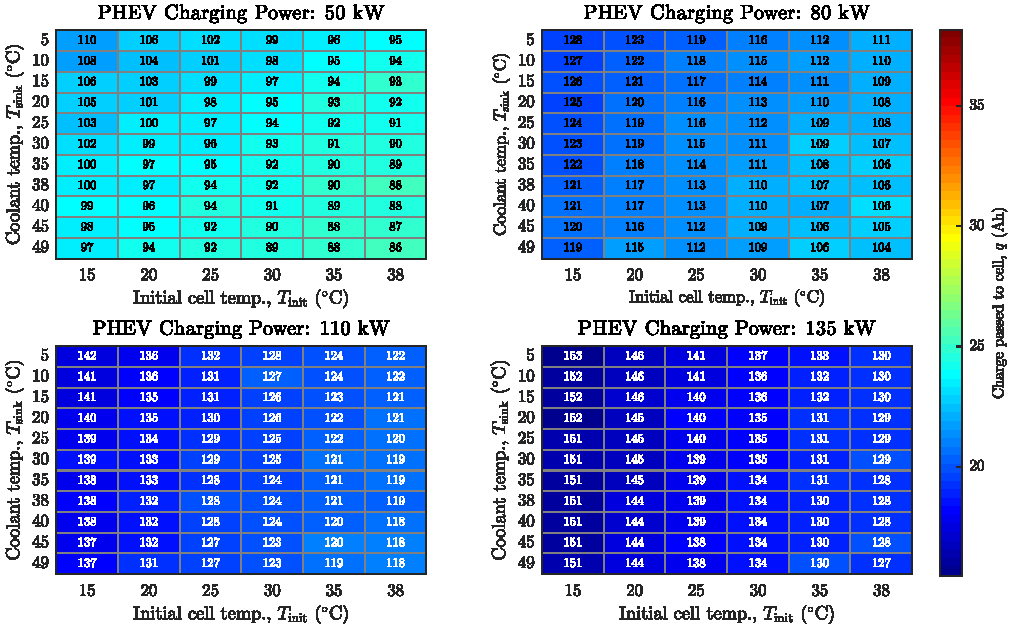
\includegraphics[width=\textwidth]{fig_generate_heatmap_PHEV}
%%        \captionsetup{labelsep=note}
%%        \caption[Optimal cell layer configurations for the \gls{phev}, presented for a range of
%%        fast charging powers and thermal conditions]{Optimal cell layer configurations for the \gls{phev}, presented for a range of
%%        fast charging powers and thermal conditions.}
%%        \label{fig:fig_generate_heatmap_PHEV}
%%        \mpfootnotes[1]
%%        \footnote{This figure was created by \mbox{Ian Campbell} who asserts copyright,
%%            with intellectual contributions from and the right to use asserted by
%%        \mbox{Krishnakumar Gopalakrishnan}.}
%%    \end{minipage}
%%\end{figure}

\subsection{Common Module Design}\label{sec:commonmodulelayeropt}

